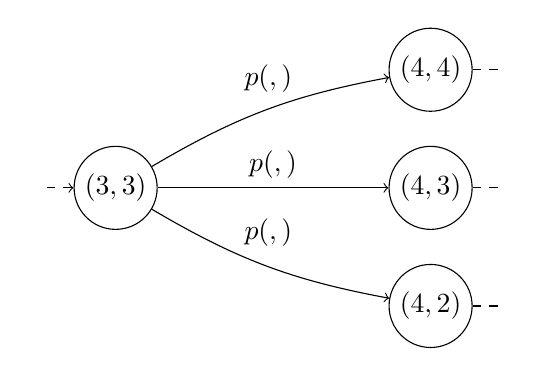
\begin{tikzpicture}[state/.style={draw,circle,inner sep=0.075cm,minimum size=1cm},scale=1.0]

  \def\spread{1.5}

  \draw (-1,0)  node[] (s00)  {};
  \draw (0,0)  node[state] (s0)  {$(3,3)$};
  \draw (4,\spread)  node[state] (s11) {$(4,4)$};
  \draw (4,0)  node[state] (s12) {$(4,3)$};
  \draw (4,-\spread) node[state] (s13) {$(4,2)$};

  \draw (5,\spread)  node[] (s21) {};
  \draw (5,0)        node[] (s22) {};
  \draw (5,-\spread) node[] (s23) {};


  \path (s0) edge[->, bend left=10, above]  node[yshift=0.10cm,xshift=0.03cm] {$p(\inc,\inc)$} (s11);
  \path (s0) edge[->, above]                node[] {$p(\inc,\pers)$} (s12);
  \path (s0) edge[->, bend right=10, above] node[yshift=0.12cm,xshift=0.03cm] {$p(\inc,\dec)$} (s13);

  \path (s00) edge[->, dashed]  node[yshift=0.10cm,xshift=0.03cm] {} (s0);
  \path (s11) edge[-, dashed]  node[yshift=0.10cm,xshift=0.03cm] {} (s21);
  \path (s12) edge[-, dashed]                node[] {} (s22);
  \path (s13) edge[-, dashed] node[yshift=0.12cm,xshift=0.03cm] {} (s23);


\end{tikzpicture}

%%% Local Variables:
%%% mode: latex
%%% TeX-master: "../paper"
%%% End:
